\documentclass[12pt,a4paper]{article}
\usepackage[utf8]{inputenc}
\usepackage[english,russian]{babel}
\usepackage{amsmath, amsfonts, amssymb, amsthm, mathtools}

\usepackage[left=20mm, top=15mm, right=15mm, bottom=20mm, nohead, nofoot]{geometry}
\usepackage{graphicx}
\usepackage{float}%"Плавающие" картинки
\usepackage{wrapfig}%Обтекание фигур (таблиц, картинок и прочего)
\usepackage{listings}
\usepackage[framed,numbered,autolinebreaks,useliterate]{mcode}


\begin{document}
	\begin{titlepage}
		
		\begin{center}	
			
			\large Санкт-Петербургский политехнический университет Петра Великого \\
			\large Физико-механический институт \\
			\large Высшая школа теоретической механики и математической физики \\[2cm] % [] - отступ
			
			\large Направление подготовки \\
			\large 01.03.03 Механика и математическое моделирование \\[4cm]
			
			
			\LARGE \textbf {Отчёт по лабораторной работе №5} \\[0.5cm] 
			\LARGE \textbf {Тема: ""Метод конечных элементов. Растяжение-сжатие упругих
				стержней"} \\[0.5cm]
			\large Дисциплина "Вычислительная механика" \\[4cm]
			
			
			
		\end{center}
		
		
		\begin{flushright} % выравнивание по правому краю
			\begin{minipage}{0.25\textwidth} % врезка в половину ширины текста
				\begin{flushleft}
					
					\large\textbf{Выполнил:}\\
					\large Работинский А.Д. \\
					\large {Группа:} 5030103/00101 \\
					
					\large \textbf{Преподаватель:}\\
					\large Е.Ю. Витохин
					
				\end{flushleft}
			\end{minipage}
		\end{flushright}
		
		
		\begin{center}
			\large Санкт-Петербург \\
			\large 2022 
		\end{center} 
		
	\end{titlepage} 
	
	\vfill % заполнить всё доступное ниже пространство
	
	\newpage
	\section{Постановка}
	Произвести расчет плоских фермы под действием нагрузки  \textbf{F}. Нагрузку следует
	прикладывать на верхний пояс. Закрепить крайне левый и правый нижний угол. Закрепление
	производится по горизонтальным и вертикальным степеням свободы. Требуется определить
	перемещения узлов фермы и усилия в стержнях.
	\begin{figure}[H]
		\centering
		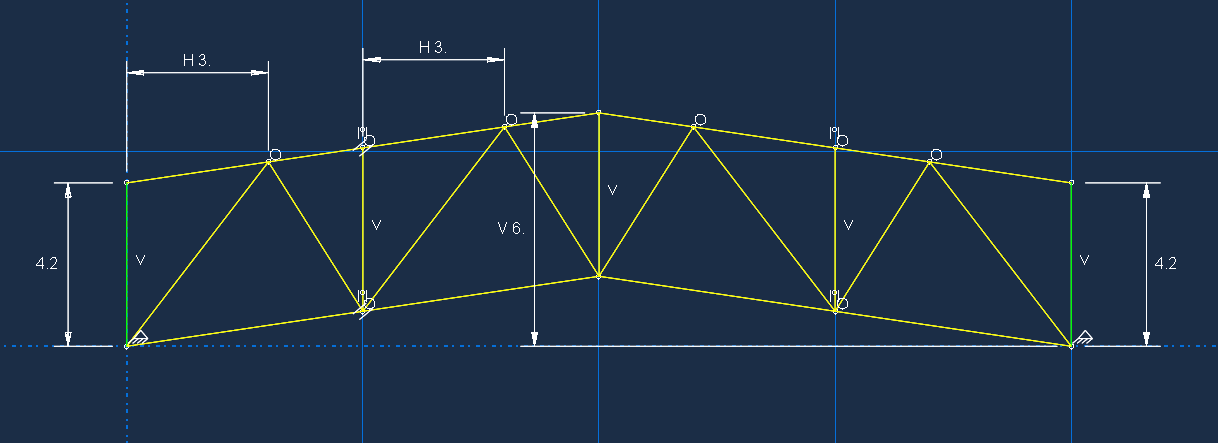
\includegraphics[width=\textwidth]{system}
		\caption{Система}
		\label{pic1}
	\end{figure}
	\section{Метод решения}
	Для решения задачи статики используется эмперический подход: минимализация функционала потенциальной энергии.\\\\
	\[
		\Pi=\Lambda-\Omega
	\]
	$\Lambda$ - энергия деформации\\	
	$\Omega$ - работа внешних сил\\
	Минимум функционала достигается в том случае, когда первая вариация этого функционала равна нулю.\\
	\[\frac{\delta\pi}{\delta \left\{U^e\right\}}=0\]
	Для каждого стержня находим локальную матрицу жесткости:\\
	\[k_{loc}^e=\frac{ES}{l}\left[\begin{array}{ccc}
		1 & -1 \\
		-1 & 1 \\
	\end{array}\right]\]
	Длину стержня находим следующим образом:
	\[l_k=(\sqrt{(x_j^k-x_i^k)^2+(y_j^k-y_i^k)^2},\] где k - номер стержня\\
	Основное уравнение МКЭ для одного элемента:
	\[\left[k^l\right]\cdot{\left\{U^l\right\}}=\left\{F^l\right\}\]
	Осуществим переход от локальной СК связанной с самим КЭ к глобальной СК при помощи матрицы перехода:
		\begin{equation*}
			T=
				\begin{bmatrix}
					l_{ij} & m_{ij} & 0 & 0 \\
					0 & 0 & l_{ij} & m_{ij} \\
				\end{bmatrix} 
		\end{equation*}
	
	Переход к матрице жесткости элемента в глобальной системе координат для каждого элемента при помощи матрицы перехода:
	\[
		k^e_{gl}=T^T\cdot k^e_{loc} \cdot T
	\], где
	\[m_{ij}=\frac{y_j-y_i}{l} \quad l_{ij}=\frac{x_j-x_i}{l}\]
	Для того, чтобы не решать систему тривиальным пересчетом, создадим глобальную матрицу жесткости, в одном конечном элементе 2 узла и в каждом 2 степени свободы, на которые накладываются соотвтсвующие жесткости), а в теле в данном случае 14 узлов, в каждом по 2 степени свободы, т.е. матрица жесткости для системы будет иметь размерность 28 на 28.Но с другой стороны:
	$\sum_{0}^{l}k_{gl}^e$
	Чтобы в результате суммирования матриц 4 на 4 получить матрицу 28 на 28 нужно задать некоторое правило по которому элемненты локальной матрицы будут записываться в глобальную матрицу для системы, очевидный для этого способ:\\
	$ u=[u_x^1,u_y^1,u_x^2,u_y^2,\dots] \Rightarrow $ если рассмотреть локальную матрицу жесткости для элемента из узлов с номерами m и n $m_x=2m-1 \quad m_y=2m \quad n_x=2n-1 \quad n_y=2n$.Далее воспользуемся способом аналогичным переводу в глобальную СК:построим некоторую матрицу А, такую что: $[A]^{T}*\left\{k_{gl}^e\right\}*[A]}$\\
	Эта матрица будет иметь следующий вид:\\
	\begin{center}
		\begin{Bmatrix}
			0&$\dots$ & 1 & 0 &$\dots$&0\\
			0&$\dots$ & 0 & 1 &$\dots$&0\\
			0&$\dots$ &$\dots$& 1 & 0&0\\
			0&$\dots$ &$\dots$& 0 & 1&0\\
		\end{Bmatrix}
	\end{center}
	
	\\
	Где ненулевые элементы стоят на местах $1;m_x \quad 2;m_y \quad 3;n_x  \quad 4;n_y$
	Преобразование такими матрицами для каждого элемента в сумме даст искомую глобальню матрицу жесткостей для системы\\
	Введем вектор сил и перемещений для системы:
	\begin{equation*}
		U=
		\begin{pmatrix}
			U_x^1 \\
			U_y^1 \\
			U_x^2\\
			U_y^2\\
			...
		\end{pmatrix}
	\qquad
	 	F=
	 	\begin{pmatrix}
	 		F_x^1 \\
	 		F_y^1 \\
	 		F_x^2\\
	 		F_y^2\\
	 		...
	 	\end{pmatrix}
	\end{equation*}
	Применим граничные условия, обнулив пары столбцов и строк и поставив единицы по диагонали у соответствующих узлов.\\
	Составим основное уравнение МКЭ:
	\begin{equation*}
		\begin{bmatrix}
			k_{11} &..&k_{1N}\\
			..&..&..\\
			k_{N1}&..&k_{NN}
		\end{bmatrix} \cdot
		\begin{pmatrix}
			U_x^1 \\
			U_y^1 \\
			U_x^2\\
			U_y^2\\
			...
		\end{pmatrix}=
		\begin{pmatrix}
			F_x^1 \\
			F_y^1 \\
			F_x^2\\
			F_y^2\\
			...
		\end{pmatrix}
	\end{equation*}
	\section{Результаты}
	\subsection{Результаты работы в Abaqus}
	\begin{figure}[H]
		\centering
		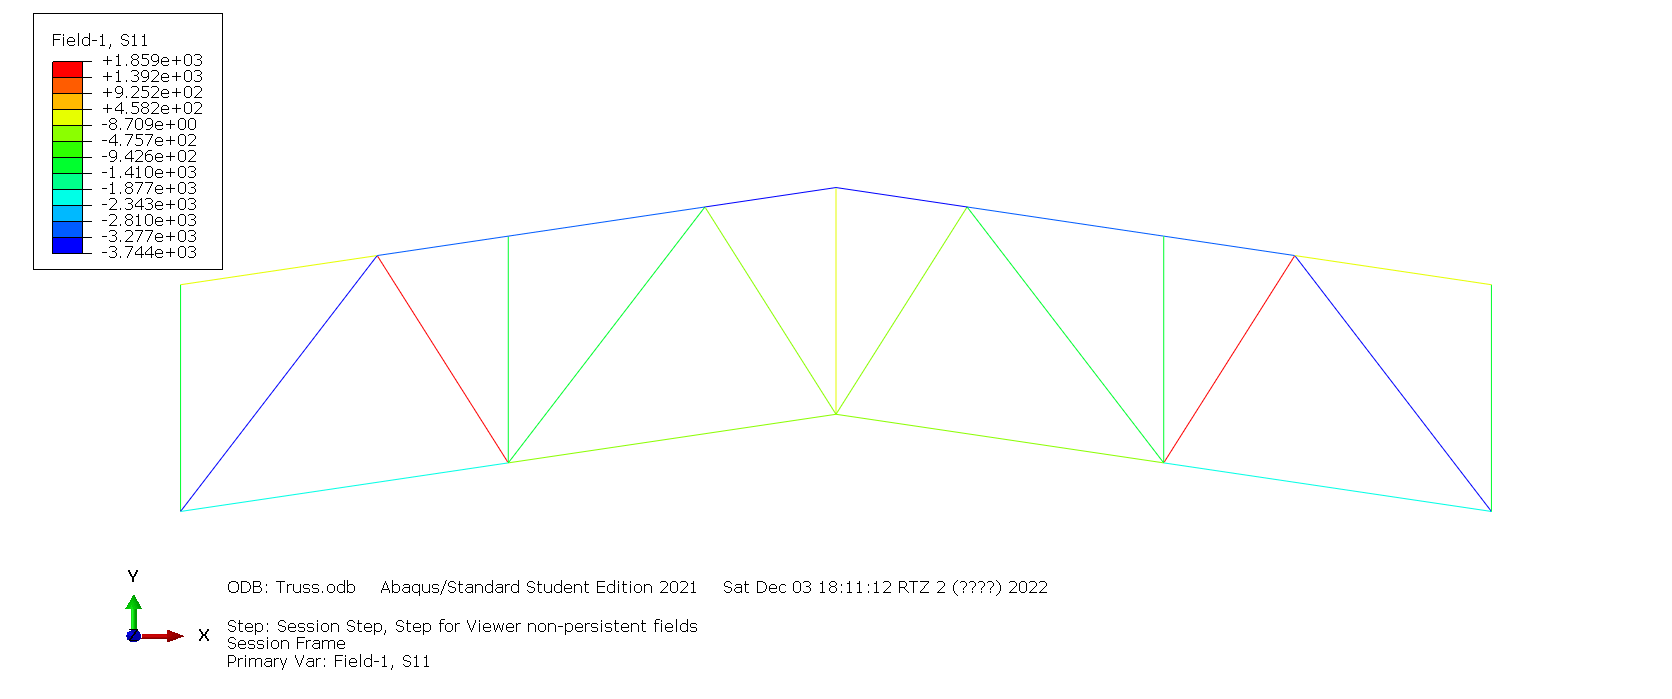
\includegraphics[width=\textwidth]{fp}
		\caption{Усилия, возникающие в ферме}
		\label{pic1}
	\end{figure}
	\begin{figure}[H]
		\centering
		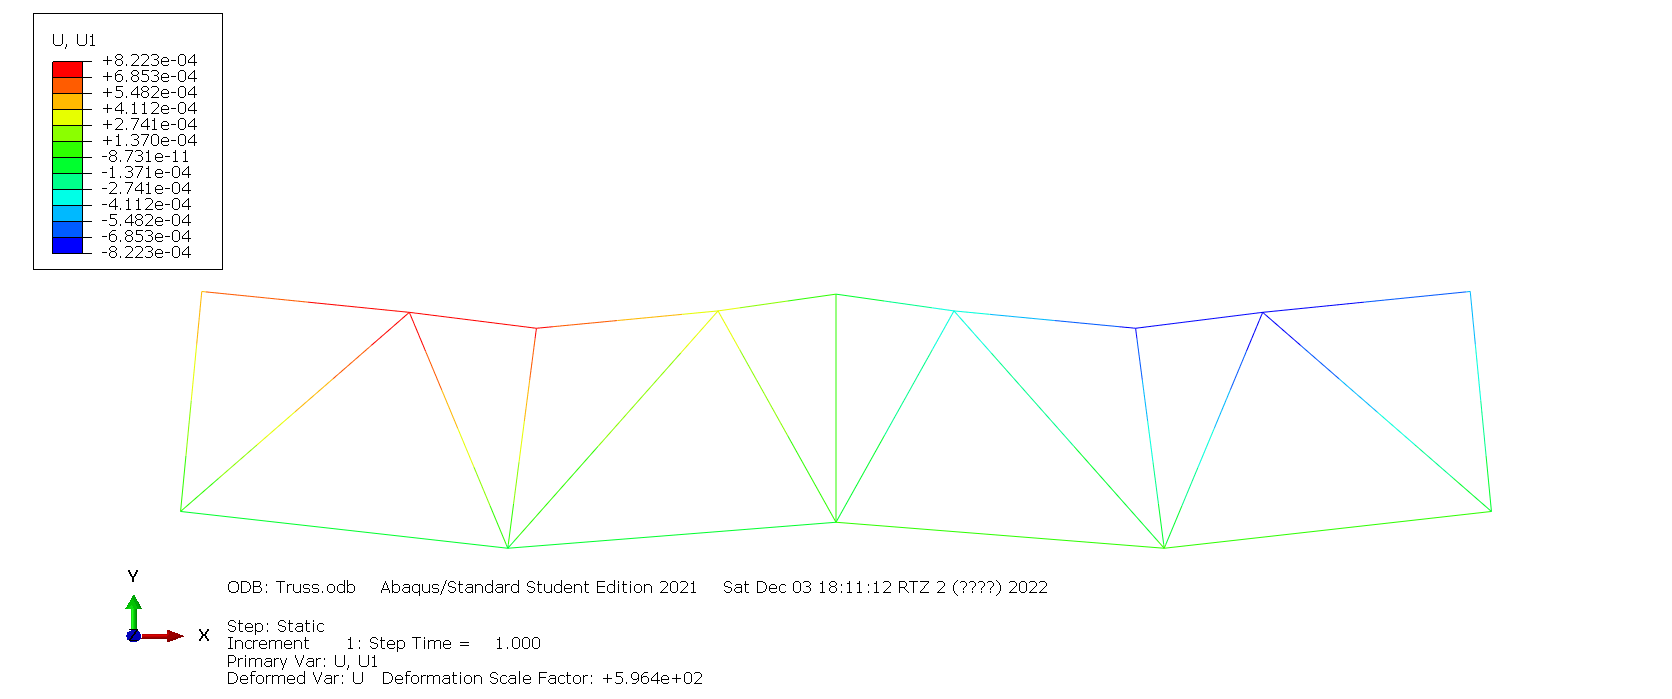
\includegraphics[width=\textwidth]{ux}
		\caption{Поле перемещений по оси Х}
		\label{pic2}
	\end{figure}
	\begin{figure}[H]
		\centering
		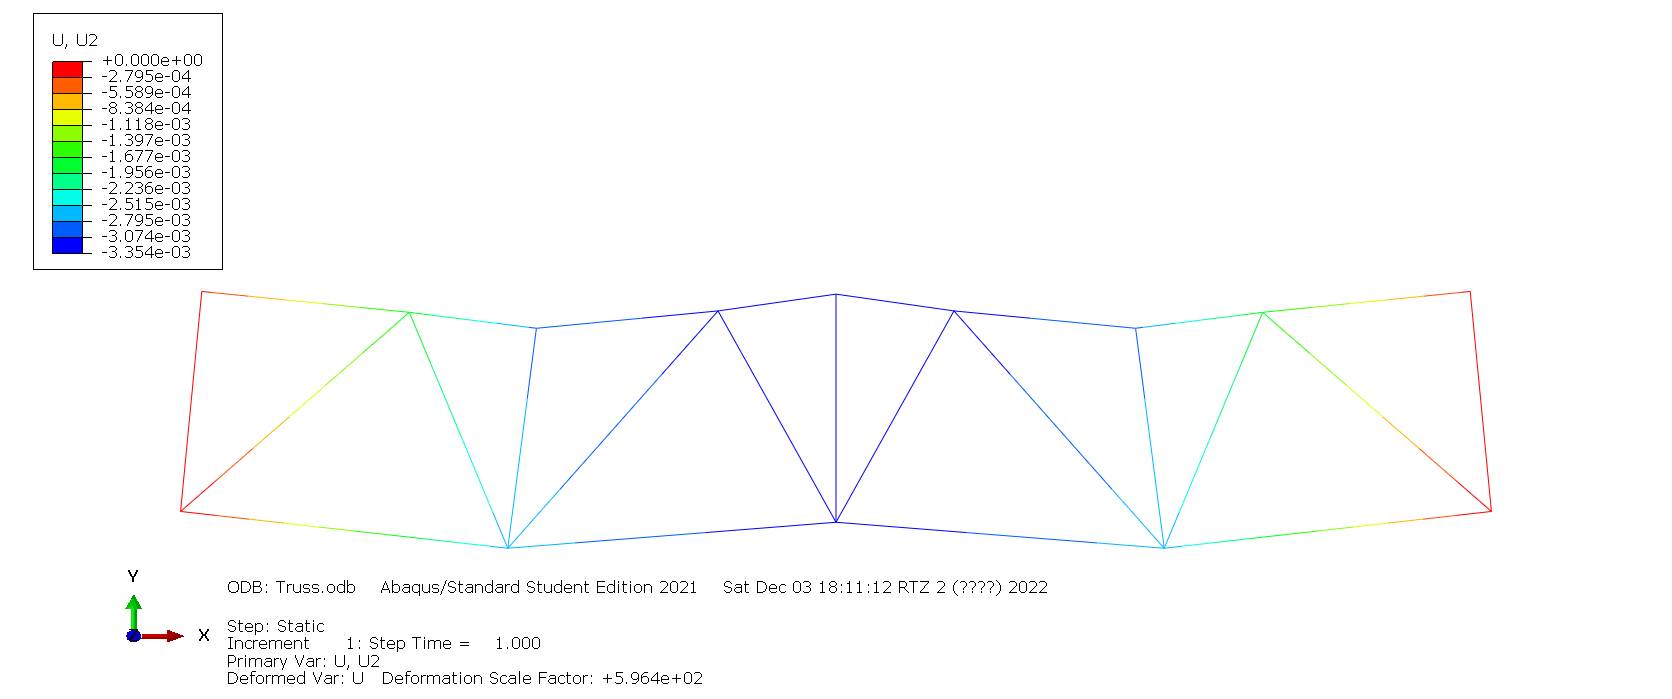
\includegraphics[width=\textwidth]{uy}
		\caption{Поле перемещений по оси Y}
		\label{pic3}
	\end{figure}
\begin{figure}[H]
	\centering
	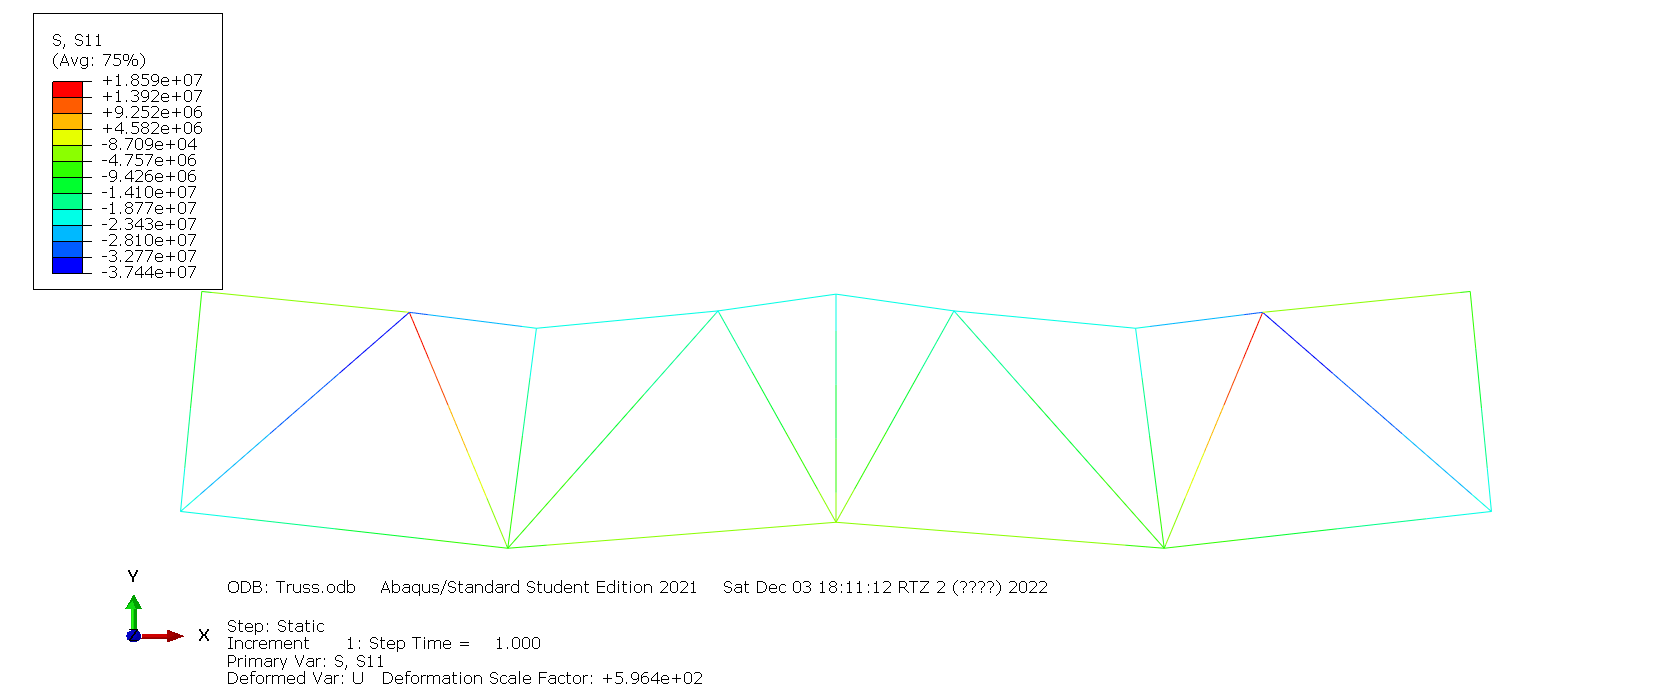
\includegraphics[width=\textwidth]{s11}
	\caption{Напряжения в ферме}
	\label{pic3}
\end{figure}
	\subsection{Результаты работы в MatLab}
\begin{figure}[H]
	\centering
	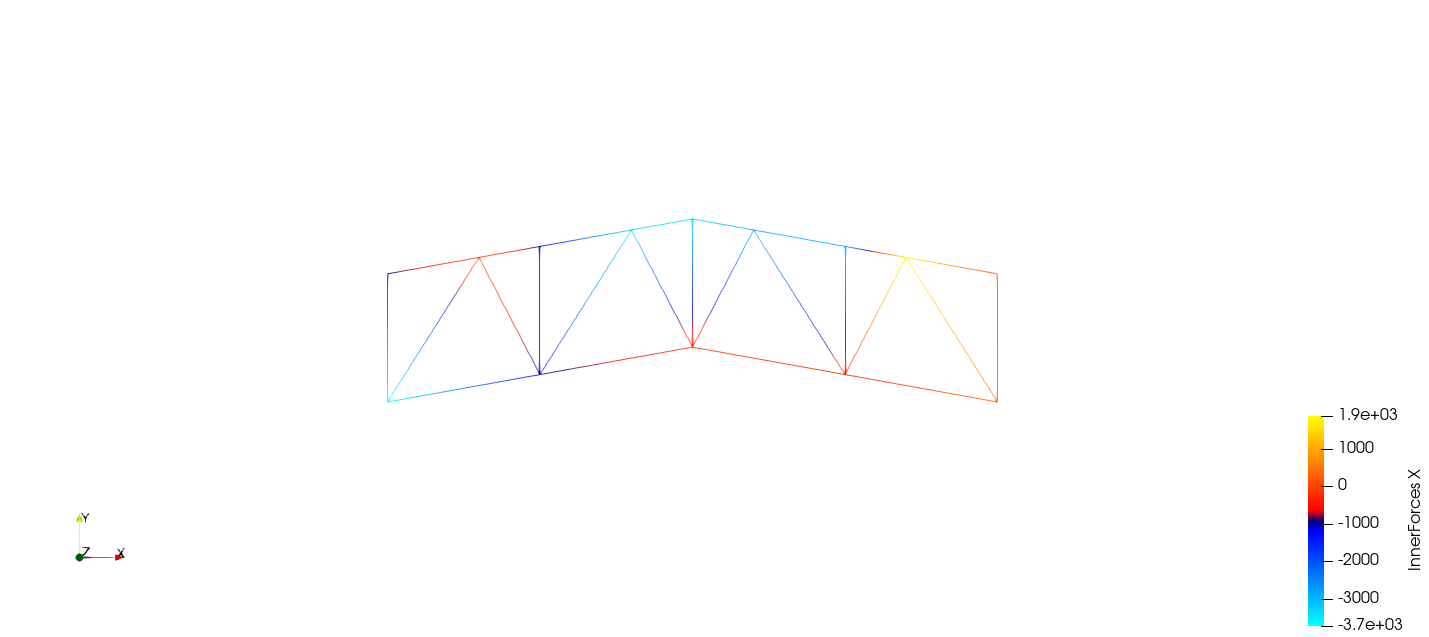
\includegraphics[width=\textwidth]{Matlab_f}
	\caption{Усилия, возникающие в ферме}
	\label{pic1}
\end{figure}
\begin{figure}[H]
	\centering
	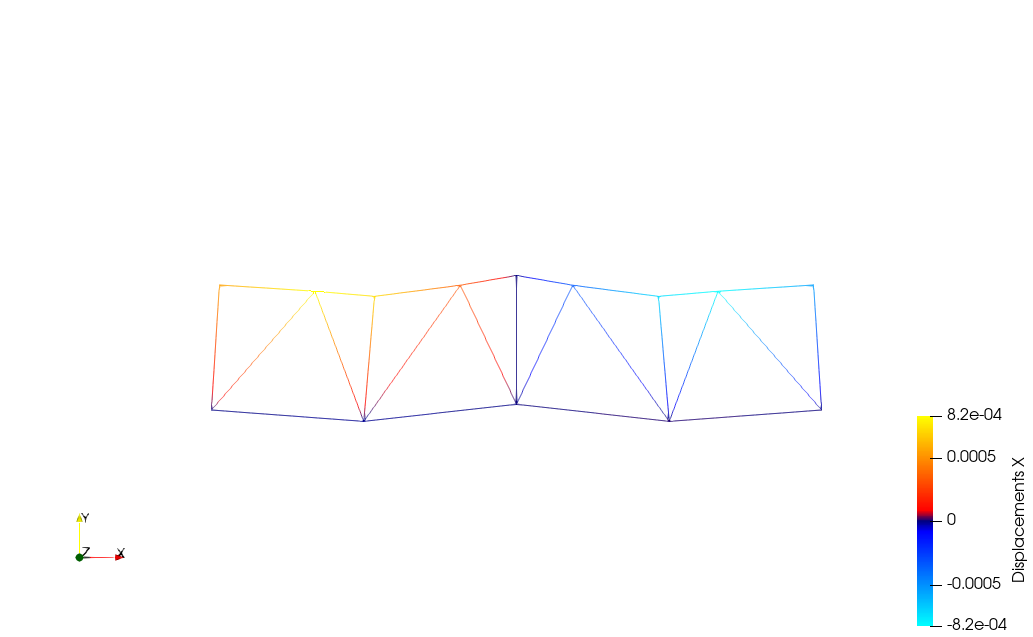
\includegraphics[width=\textwidth]{Matlab_ux}
	\caption{Поле перемещений по оси Х}
	\label{pic2}
\end{figure}
\begin{figure}[H]
	\centering
	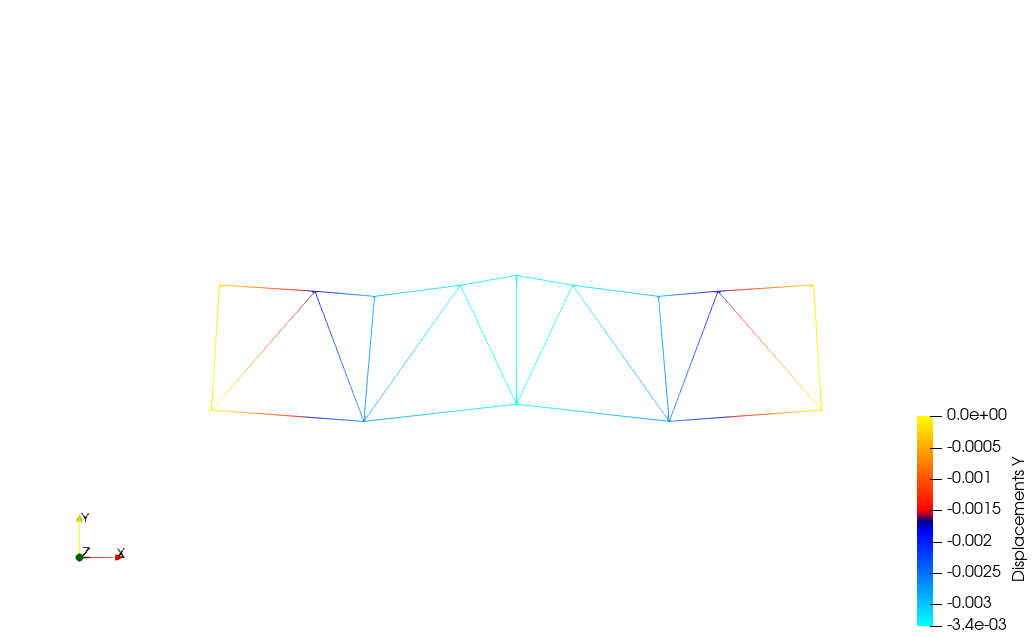
\includegraphics[width=\textwidth]{Matlab_uy}
	\caption{Поле перемещений по оси Y}
	\label{pic3}
\end{figure}
	\subsection{Сравнение результатов}
	\begin{figure}[H]
		\centering
		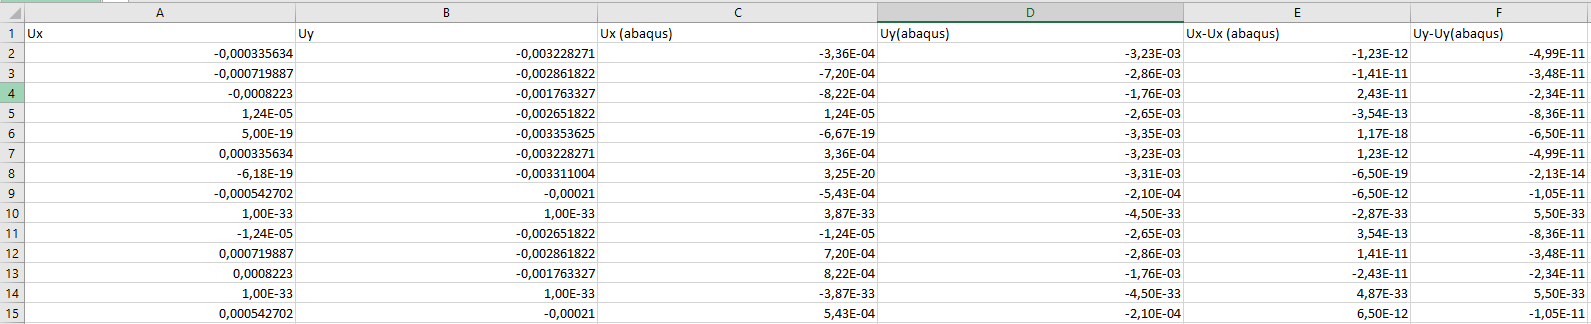
\includegraphics[scale=0.4]{compare_u}
		\caption{Сравнение результатрв для перемещений}
		\label{pic7}
	\end{figure}
	\begin{figure}[H]
		\centering
		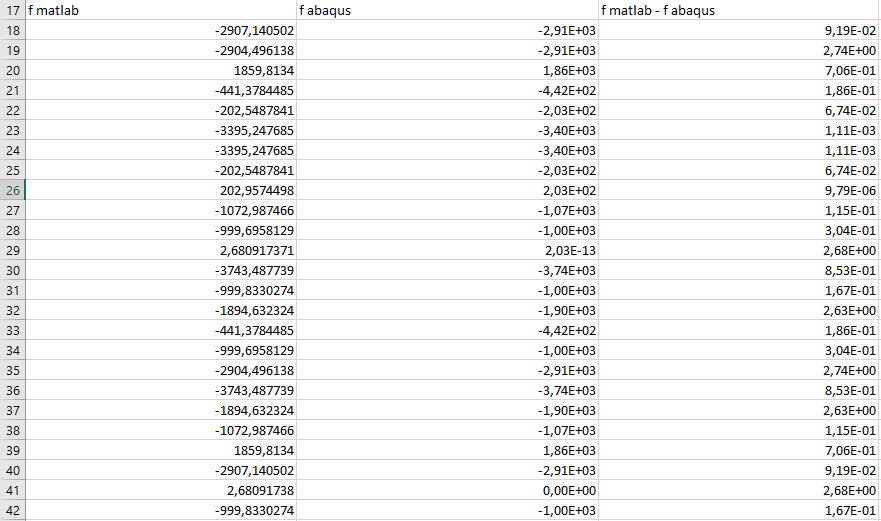
\includegraphics[scale=0.6]{compare_f}
		\caption{Сравнение результатов для сил}
		\label{pic8}
	\end{figure}
\section*{Выводы}
	Заметим, что  перемещения вычисленные в Абакусе и в МатЛабе в среднем различаются в 10-13 знаках,а силы различаются в среднем в 1-2 знаке, что подтверждает верность полученных результатов.
\end{document}
